\documentclass{article}
\usepackage{ctex}
\usepackage{bm}
\usepackage[colorlinks, linkcolor=blue]{hyperref}
\usepackage{geometry}
\geometry{left=3cm, right=3cm, top=3cm, bottom=3cm}
\usepackage{amsmath}
\usepackage{amsthm}
\usepackage[T1]{fontenc}
\usepackage{xcolor}
\usepackage{lmodern}
\usepackage{listings}

\newtheorem{task}{问题}

\lstset{
	numbers=left, 
	numberstyle= \small, 
	keywordstyle= \color{ blue!70},
	commentstyle= \color{red!50!green!50!blue!50}, 
	frame=shadowbox, % 阴影效果
	showstringspaces = false,
	flexiblecolumns,                % 别问为什么,加上这个
	rulesepcolor= \color{ red!20!green!20!blue!20} ,
	escapeinside=``, % 英文分号中可写入中文
	breaklines=true,
	%xleftmargin=2em,xrightmargin=2em, aboveskip=1em,
	framexleftmargin=2.7em
}

\lstdefinestyle{Fortran}{
	language        =   [90]Fortran,
	basicstyle=\small\ttfamily
}

\title{作业二:非线性方程求根}
\author{英才1701 赵鹏威 U201710152}

\begin{document}
	\maketitle
	\tableofcontents
	\newpage
	\section{引言}
	在物理中会遇到很多方程求根的问题,一般这些方程是非线性的,甚至是超越方程. 另外,方程求根问题实际上就是求函数的零点,这也对应着求函数极值点的问题. 因此开发有效的数值求根方法是很有必要的. 常用的算法有:二分法、Jacobi 迭代法、牛顿下山法. 为了让 Jacobi 迭代法收敛更快,又有人提出了事后加速法、Atiken 加速法. 这次作业就是通过 Fortran 来实现这些算法. 
	
	\section{问题描述}
	\begin{task}
		使用不同的算法求非线性方程
		\[
		f(x)=\frac{x^3}{3}-x=0
		\]
		的根,并比较它们的性能,包括:结果的准确性、误差大小、迭代次数
	\end{task}
	
	这是一个一元三次方程,很容易得到这个方程的解析解
	\[
	x_1 = -\sqrt{3}\approx-1.732051 \quad x_2 = 0 \quad x_3=\sqrt{3}\approx1.732051.
	\]
	这里将解析解四舍五入到了精确到6位小数的数值,之后会将由算法得到的结果与这个结果来比较,验证算法的准确性.
	
	\section{程序实现}
	希望程序达到的效果是:向程序提供函数$f(x)$(和迭代式$\varphi(x)$,如果有的话),区间$[a, b]$,程序可以调用某种指定的算法,在指定的精度下,找出这个区间内所有可能的根. 
	
	为了达到这个目的,通过两步来实现整个程序. 第一步是将每种算法分别单独写成一个 subroutine,这些 subroutine 以函数 $f$,迭代式 $\varphi$,初值(对二分法来说是初始的区间)和要求的精度为输入参数,返回最多一个找到的根. 第二步是另写一个 subroutine 作为调用这些算法的接口程序,它的作用是将输入的区间等分成若干个小区间,然后调用第一步中的子程序在这些小区间内寻找根,并且对于方便预先判断收敛性的算法,在调用之前会自动判断这个区间内的迭代是否一定会收敛,跳过不一定收敛的区间,这样可以省去很多不必要的计算.
	
	下面详细阐述实现细节.
	
	\subsection{辅助模块}
	这个模块存放一些对程序实现有帮助但不是必须的东西,包括一些常数、新的类型定义和一些函数.
	\subsubsection{result 类型}
	由于几乎在所有的情况下,数值计算的结果具有一定的误差,所以可以定义一个 result 类型,将计算结果和误差封装在一起储存.
	\lstinputlisting[
	style = Fortran,
	caption     =   {\bf result 类型},
	label       =   {result_type.f90}
	]{./utils/snips/result_type.f90}
	\subsubsection{数值导数}\label{sbbs:numerical_derivative}
	一些程序里需要求导数,比如牛顿下山法,因此写一个 function 来实现数值导数的功能. 这样计算的导数必然会有误差,但是可以证明这些误差不会累加到最后的结果上.
	\lstinputlisting[
	style = Fortran,
	caption     =   {\bf 数值导数},
	label       =   {numerical_derivative.f90}
	]{./utils/snips/numerical_derivative.f90}
	\subsubsection{判断是否一定收敛}
	Jacobi 迭代法以及对应的加速方法都可以提前判断迭代是否会收敛. 为了节约计算资源,在迭代前对迭代是否收敛进行判断. 根据理论,只要迭代函数$\varphi(x)$在区间$[a, b]$满足下面两个条件就可以保证迭代一定会收敛:
	\begin{itemize}
		\item $\forall x\in[a, b],\;\varphi(x)\in[a, b]$
		\item $\exists L<1\forall x\in[a, b],\;|\varphi'(x)|\le L$
	\end{itemize}
	要实现收敛性的判断需要知道$\varphi(x)$和它的导数$\varphi'(x)$在区间$[a,b]$上的取值范围,这里使用最直接的方法,也就是将区间均匀分成一些各点,计算$\varphi(x)$和它的导数$\varphi'(x)$在这些点上的值,取最大值和最小值作为函数在这个区间的上下限. 
	\lstinputlisting[
	style = Fortran,
	caption     =   {\bf 收敛性预判断},
	label       =   {convergence_check.f90}
	]{./utils/snips/convergence_check.f90}
	\subsection{求根的主要算法}
	将二分法、Jacobi迭代法、牛顿下山法、事后加速法和Atiken加速法封装到一个模块里. 每种方法都用 subroutine 实现,如二分法,输入函数、区间和精度,返回满足精度要求的结果.
	\lstinputlisting[
	style = Fortran,
	caption     =   {\bf 二分法},
	label       =   {bisection.f90}
	]{./utils/snips/bisection.f90}
	其他方法的实现大同小异,为了文章的简洁,源码见附录(Jacobi 迭代法:第169行,牛顿下山法:第216行,事后加速法:第272行,Atiken:第320行). 需要注意的是,这些子程序都最多只能找到一个根. 另外有一些值得说明一下的细节
	\begin{itemize}
		\item 牛顿下山法中的参数$\lambda$在每次迭代前会恢复为1;
		\item 牛顿下山法中计算导数使用数值导数(\ref{sbbs:numerical_derivative}节);
		\item 事后加速法中第$n$次迭代使用的$L$取的是当前位置导数值$\varphi'(x_n)$,同样用数值导数.
	\end{itemize}
	\subsection{接口子程序与区间扫描}
	上面实现的方法只能找到一个根,但是我们希望的是尽可能一次性找出所有可能的根. 可以采用这样的做法,给定一个区间$[a, b]$,将这个区间等分成若干个小区间,在这些小区间里调用上面写的各种求根算法的子程序. 如果使用的方法为 Jacobi 迭代、事后加速法和 Atiken 法,那么在调用求根子程序前先判断在这个小区间内能否一定收敛,如果是的话才调用程序. 这样就可以找出一个较大的区间内的所有可能的根. 将上面所述的区间扫描功能写在一个 subroutine 内,这个 subroutine 作为调用求根函数的接口. 它的功能可以用下面的流程图表示,见图\ref{fig:multi_seeker}. 代码见附录第532行.
	\begin{figure}[h!tb]
		\centering
		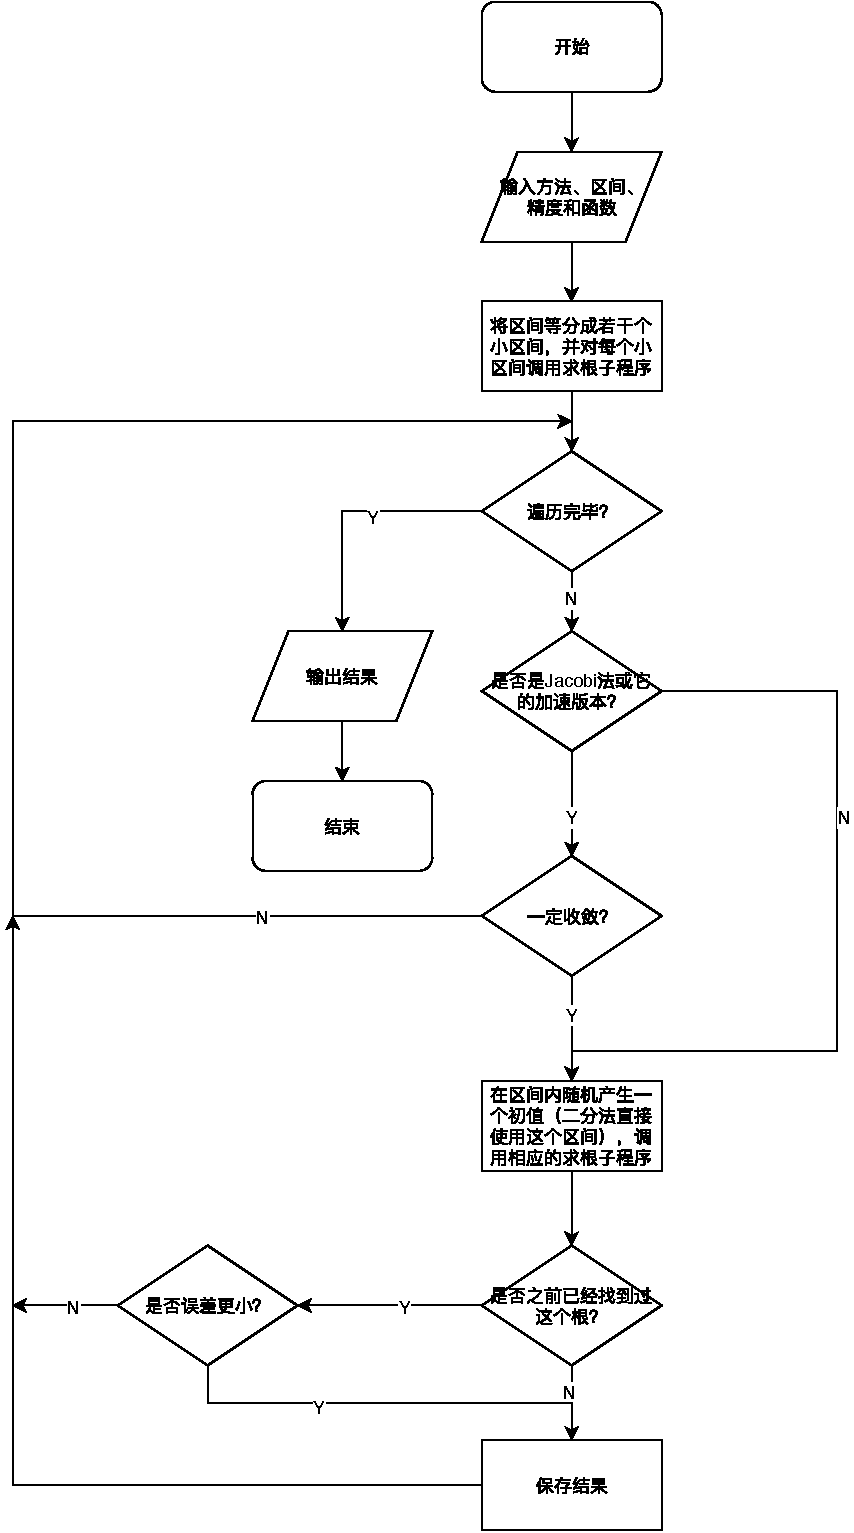
\includegraphics[width=0.5\textwidth]{./utils/multi_seeker.pdf}
		\caption{ 接口子程序的流程图\label{fig:multi_seeker}}
	\end{figure}
	\section{运行时结果}
	下面各方法要求的精度为
	\[
	\begin{split}
		|x_k-x_{k-1}|&\le 10^{-5} \\
		|f(x_k)|&\le 10^{-5}
	\end{split}
	\]
	输入的区间为$[-10, 10]$.
	\subsection{二分法}
	主程序代码如下
	\lstinputlisting[
	style = Fortran,
	caption     =   {\bf 二分法主程序},
	label       =   {main_bisection.f90}
	]{./utils/snips/main_bisection.f90}
	结果如图\ref{fig:rtr_bisection}所示. 求得的结果为(取到第6位小数)
	\[
	\begin{split}
	x_1&=-1.732053(6) \\
	x_2&=0.000003(6) \\
	x_3&=1.732053(6)
	\end{split}
	\]
	括号内为最后一位误差. 可见与准确的结果符合.
	\begin{figure}[htb]
		\centering
		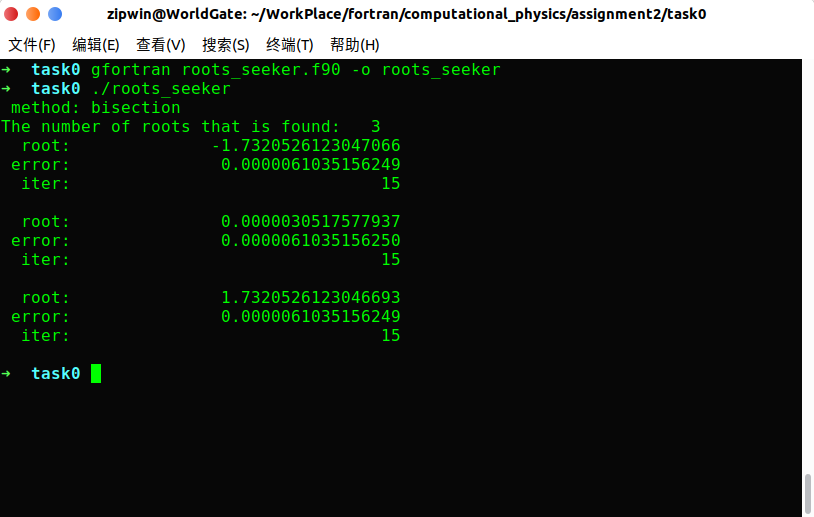
\includegraphics[width=0.85\textwidth]{./utils/rtr_bisection.png}
		\caption{ 二分法\label{fig:rtr_bisection}}
	\end{figure}
	\subsection{Jacobi 迭代法}
	主程序如下
	\lstinputlisting[
	style = Fortran,
	caption     =   {\bf Jacobi 迭代法主程序},
	label       =   {jacobi.f90}
	]{./utils/snips/main_jacobi.f90}
	Jacobi 迭代法使用了两个迭代函数
	\[
	\varphi_1(x)=(3x)^\frac{1}{3},\quad\varphi_2(x)=\frac{x^3}{3}
	\]
	运行的结果如图\ref{fig:rtr_jacobi}所示. 结果为
	\[
	\begin{split}
	x_1&=-1.732053(5) \\
	x_2&=0.000000(0) \\
	x_3&=1.732048(5)
	\end{split}
	\]
	其中$x_1,x_3$是使用$\varphi_1(x)=(3x)^{1/3}$得到的,$x_2$是使用$\varphi_2(x)=x^3/3$得到的.
	\begin{figure}[htb]
		\centering
		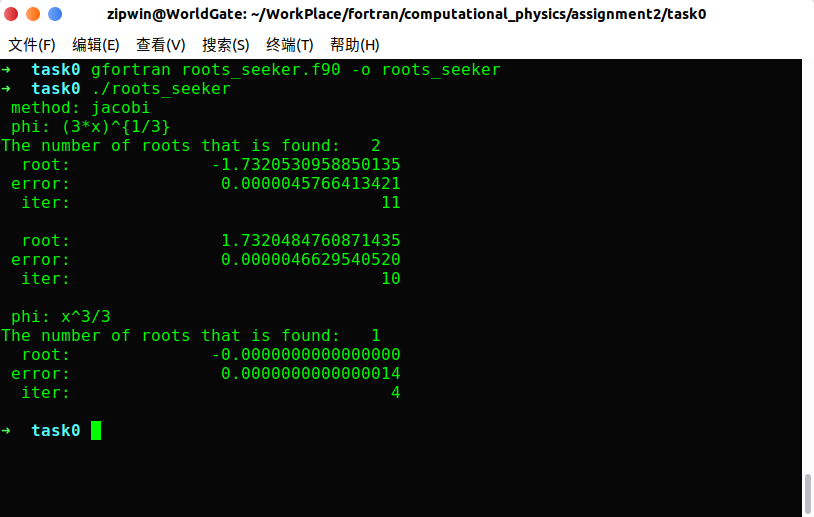
\includegraphics[width=0.85\textwidth]{./utils/rtr_jacobi.png}
		\caption{ Jacobi迭代法\label{fig:rtr_jacobi}}
	\end{figure}
	\subsection{牛顿下山法}
	主程序如下
	\lstinputlisting[
	style = Fortran,
	caption     =   {\bf 牛顿法主程序},
	label       =   {downhill.f90}
	]{./utils/snips/main_downhill.f90}
	运行结果如图\ref{fig:rtr_downhill}所示. 结果为
	\[
	\begin{split}
	x_1&=-1.732051(0) \\
	x_2&=0.000000(0) \\
	x_3&=1.732051(0)
	\end{split}
	\]
	可见牛顿下山法的精度非常高.
	\begin{figure}[htb]
		\centering
		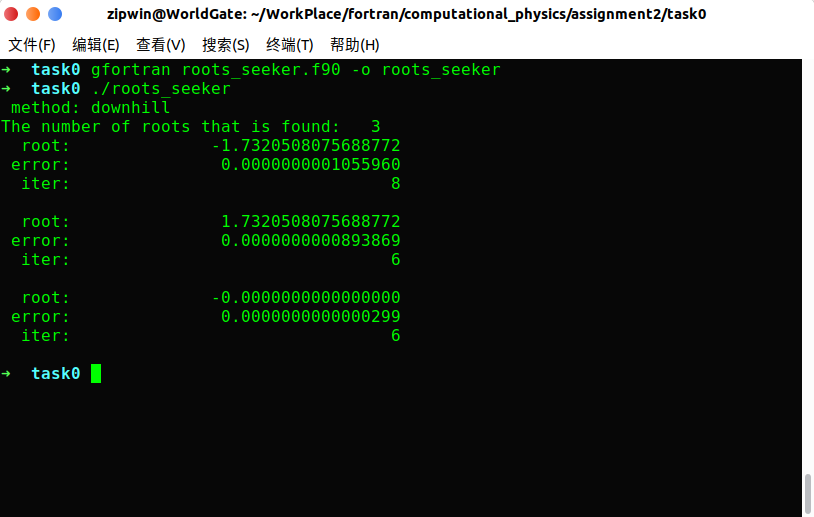
\includegraphics[width=0.85\textwidth]{./utils/rtr_downhill.png}
		\caption{ 牛顿下山法\label{fig:rtr_downhill}}
	\end{figure}
	
	\subsection{事后加速法}
	主程序如下
	\lstinputlisting[
	style = Fortran,
	caption     =   {\bf 事后加速法主程序},
	label       =   {post.f90}
	]{./utils/snips/main_post.f90}
	运行结果如图\ref{fig:rtr_post}所示. 结果为
	\[
	\begin{split}
	x_1&=-1.732051(0) \\
	x_2&=0.000000(0) \\
	x_3&=1.732051(0)
	\end{split}
	\]
	\begin{figure}[htb]
		\centering
		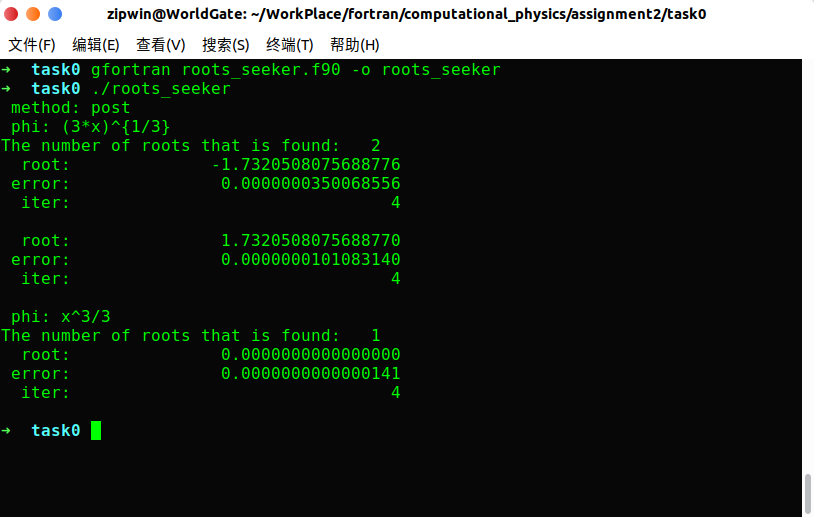
\includegraphics[width=0.85\textwidth]{./utils/rtr_post.png}
		\caption{ 事后加速法\label{fig:rtr_post}}
	\end{figure}
	
	\subsection{Atiken 法}
	主程序如下
	\lstinputlisting[
	style = Fortran,
	caption     =   {\bf Atiken 法主程序},
	label       =   {atiken.f90}
	]{./utils/snips/main_atiken.f90}
	运行结果如图\ref{fig:rtr_atiken}所示. 结果为
	\[
	\begin{split}
	x_1&=-1.732051(0) \\
	x_2&=0.000000(0) \\
	x_3&=1.732051(0)
	\end{split}
	\]
	\begin{figure}[h!tb]
		\centering
		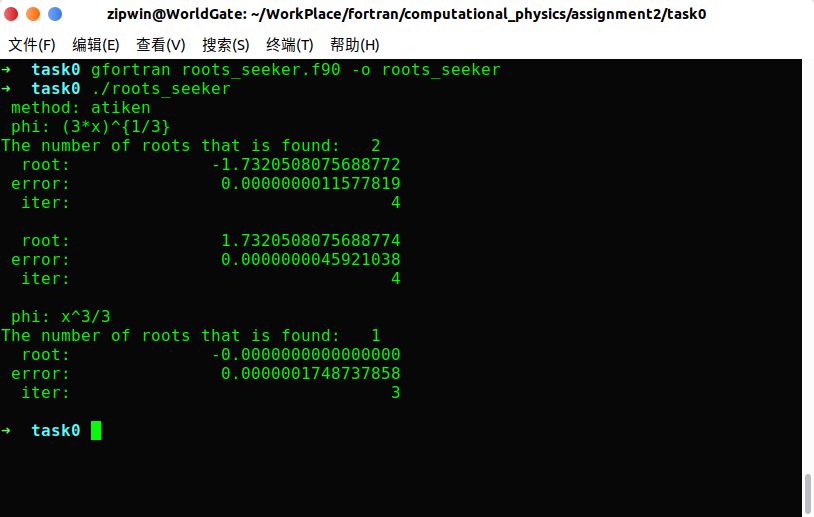
\includegraphics[width=0.85\textwidth]{./utils/rtr_atiken.png}
		\caption{ Atiken 法\label{fig:rtr_atiken}}
	\end{figure}
	
	\section{各方法的比较}
	从上面的运行结果可以发现,牛顿下山法的精度最高,要求的精度为$10^{-5}$,而牛顿下山法达到了$10^{-11}$以上的精度. 事后加速法和 Atiken 法次之. 而二分法可以很好地控制精度. 至于收敛速度,从上面的结果也可以发现,二分法最慢,Jacobi 法稍快一些,牛顿下山法、事后加速法和 Atiken 法收敛速度较快. 进一步比较收敛速度,让这几种方法都以$3.0$为初值(二分法为$[1.0, 4.0]$),迭代30次,收敛曲线如图\ref{fig:compare}所示. 可见最快的算法是 Atiken 法. 而二分法出现震荡,收敛最慢.
	\begin{figure}[h!tb]
		\centering
		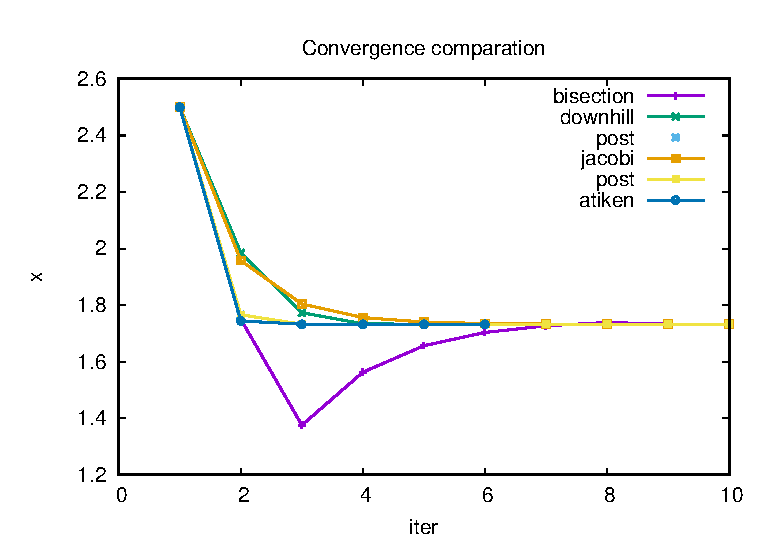
\includegraphics[width=0.7\textwidth]{./utils/compare.eps}
		\caption{ 各方法收敛速度的比较\label{fig:compare}}
	\end{figure}
	
	\newpage
	\section*{附录}
	代码可在\url{https://github.com/ZipWin/computational_physics/tree/master/assignments/assignment2}找到.
	\lstinputlisting[
	style = Fortran,
	caption     =   {\bf roots\_seeker.f90},
	label       =   {roots_seeker.f90}
	]{./utils/roots_seeker.f90}
	
	
\end{document}